% File: ot-extension-ladder.tex
% See also file: ot-step-ladder.tex

\documentclass{standalone}

% preamble for jupiter-paper related TikZ drawing
\usepackage{tikz}
\usetikzlibrary{shapes, positioning, arrows.meta, calc, backgrounds, fit}

% default horizontal/vertical distance
\def\hdist{1.5}
\def\vdist{1.5}

\newcommand{\state}[2]{% #1: state label; #2: position
  \node (#1) [circle, inner sep = 0pt, minimum size = 10mm, text width = 10mm, align = center, draw, #2, font = \Large] {$#1$};
}

\newcommand{\transition}[4][]{% #2: start state; #3: end state; #4: transition label; #1: transition label position (optional)
  \draw[>=Stealth, ->] (#2) to node [rectangle, draw, above = 2pt, sloped, #1] {#4} (#3);
}

\tikzset{node distance = \vdist and \hdist}
\tikzset{path/.style = {draw, rounded corners, very thick, #1}}


\newcommand{\stateN}[2]{% #1: state label; #2: position
  \node (#1) [circle, inner sep = 0pt, minimum size = 10mm, text width = 10mm, align = center, draw, #2, font = \Large] {};
}

\begin{document}
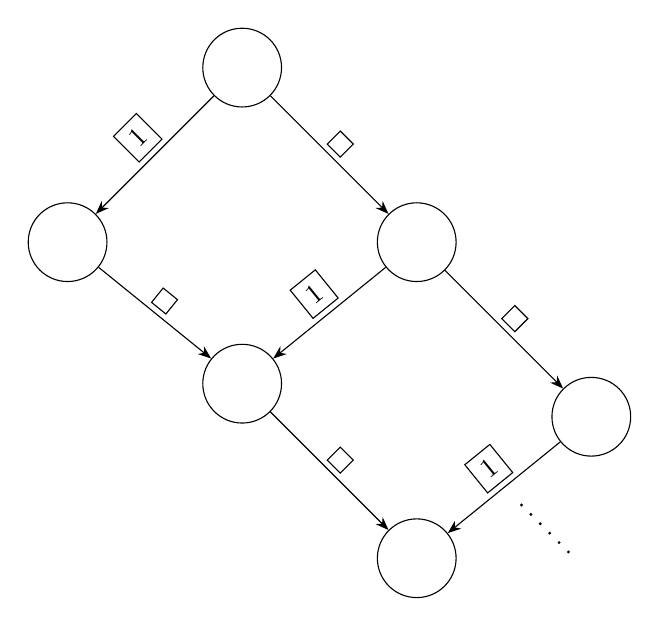
\begin{tikzpicture}
  \stateN{0}{}
  \stateN{1}{below left = of 0}
  \stateN{2}{below right = of 0}
  \stateN{12}{below = 2.0*\vdist of 0}

  \transition{0}{1}{1}
  \transition{0}{2}{}
  \transition{1}{12}{}
  \transition{2}{12}{1}

  \stateN{23}{below right = of 2}
  \stateN{123}{below right = of 12}

  \transition{2}{23}{}
  \transition{12}{123}{}
  \transition{23}{123}{1}

  \coordinate (c) at ($(23)!0.5!(123)$);
  \draw[loosely dotted, thick] ($(c) + (-45:0.30cm)$) to ++(-45:1.0cm);
\end{tikzpicture}
\end{document}
